\begin{frame}
    \begin{minipage}{0.45\textwidth}
        \textbf{\underline{Second Approach} - Video Embedding:}

        \vspace{0.5em}

        We'll use the S3D \cite{S3d} model.

        \begin{itemize}
            \item Trained on HowTo100M dataset.
            \item Intended for video retrieval / search.
            \item Produces embeddings of size 1024.
        \end{itemize}

    \end{minipage}
    \hfill
    \begin{minipage}{0.45\textwidth}
        \centering
        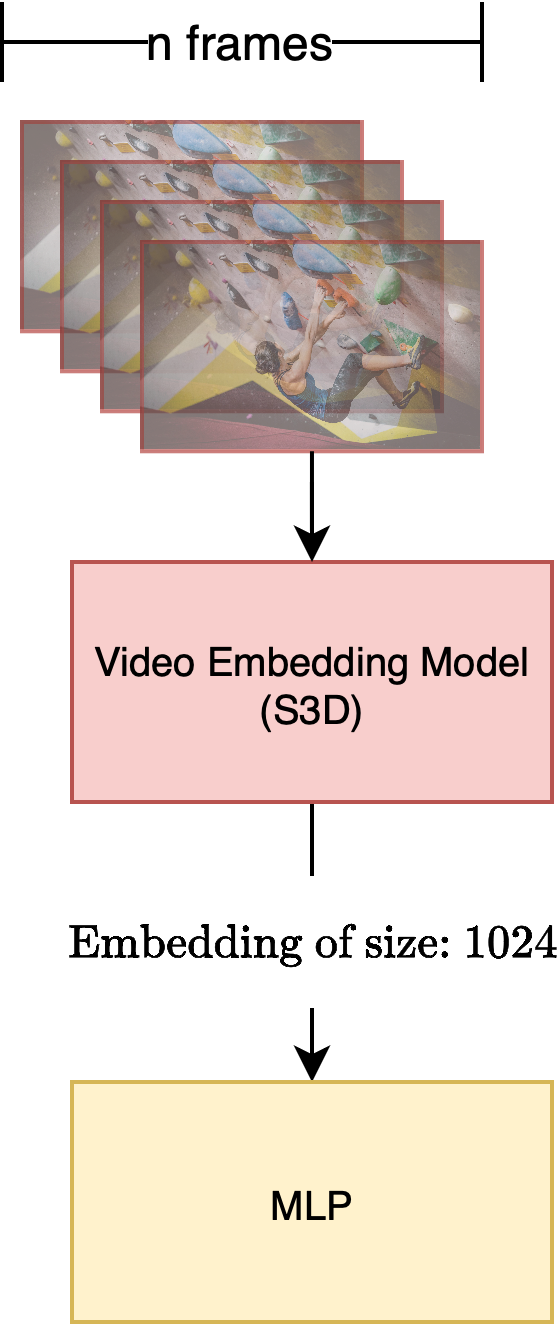
\includegraphics[width=0.45\textwidth]{assets/visuals/video-embedding-approach.drawio.png} % Adjusted width

    \end{minipage}
\end{frame}

% NOTE: say that our hypothesis was that using these features we could attain some results and in fact we observed a sort of improvement in the accuracy.
% NOTE: we have chosen this approach because of the embedding.
% NOTE: results justifications, maybe because the HowTo100M dataset on which the model was trained on wasn't really meant for video classification but more for effective video retrieval and search.